\documentclass[11pt,a4paper]{article}

%==================== Packages ====================
\usepackage[T1]{fontenc}
\usepackage[utf8]{inputenc}
\usepackage{lmodern}
\usepackage[scaled=0.92]{zi4}            % Inconsolata for code
\usepackage[margin=2.2cm,top=2.6cm,headheight=14pt]{geometry}
\usepackage[table]{xcolor}
\usepackage{listings}
\usepackage[most]{tcolorbox}
\usepackage{tabularx,array}
\usepackage{enumitem}
\usepackage{titlesec}
\usepackage{fancyhdr}
\usepackage{tikz}
\usetikzlibrary{positioning,arrows.meta,shadows}
\usepackage{parskip}
\PassOptionsToPackage{obeyspaces,spaces}{url}
\usepackage{hyperref}

%==================== Colours ====================
\definecolor{primary}{HTML}{0B3C5D}
\definecolor{accent}{HTML}{1D9A96}
\definecolor{accentlight}{HTML}{E6F4F3}
\definecolor{warn}{HTML}{D9822B}
\definecolor{warnlight}{HTML}{FDF1E5}
\definecolor{tipc}{HTML}{3A7D44}
\definecolor{tiplight}{HTML}{EAF5EC}
\definecolor{rowalt}{HTML}{F3F6F9}
\definecolor{inlinecode}{HTML}{B23A48}
% terminal (One Dark-like)
\definecolor{termbg}{HTML}{282C34}
\definecolor{termbar}{HTML}{1F2329}
\definecolor{termfg}{HTML}{ABB2BF}
\definecolor{termkw}{HTML}{C678DD}
\definecolor{termcmd}{HTML}{61AFEF}
\definecolor{termstr}{HTML}{98C379}
\definecolor{termcom}{HTML}{8B93A1}
\definecolor{termvar}{HTML}{E5C07B}
\definecolor{termnum}{HTML}{D19A66}

\hypersetup{colorlinks=true,linkcolor=primary,urlcolor=accent}

%==================== Inline code & keys ====================
\DeclareUrlCommand\cmd{\def\UrlFont{\ttfamily\color{inlinecode}}}
\makeatletter
\g@addto@macro\UrlBreaks{\do\_\do\-\do\=}
\makeatother
\newtcbox{\kbd}{on line, boxsep=0pt, left=3pt, right=3pt, top=1.5pt, bottom=1.5pt,
  colback=gray!8, colframe=gray!55, boxrule=0.5pt, arc=2pt,
  fontupper=\sffamily\footnotesize\bfseries}

%==================== Code listings ====================
\lstdefinestyle{bashdark}{
  language=bash,
  basicstyle=\ttfamily\small\color{termfg},
  keywordstyle=\color{termkw}\bfseries,
  emphstyle=\color{termcmd},
  commentstyle=\color{termcom}\itshape,
  stringstyle=\color{termstr},
  morekeywords={local,source,set,read,unset,return,seq},
  emph={sudo,tmux,curl,jq,docker,make,python3,pgrep,pkill,tee,mkdir,
        sleep,printf,xdg-open,date,dirname,basename,grep,pip},
  morestring=[b]",
  morestring=[b]',
  numbers=none,
  columns=fullflexible,
  keepspaces=true,
  breaklines=true,
  postbreak=\mbox{\textcolor{termcom}{$\hookrightarrow$}\space},
  showstringspaces=false,
  upquote=true,
  literate={\$}{{\textcolor{termvar}{\$}}}1
}
\lstdefinestyle{bashdarknum}{
  style=bashdark,
  numbers=left,
  numberstyle=\tiny\color{termcom},
  numbersep=8pt,
  xleftmargin=14pt
}

% Terminal box with a "title bar" and traffic-light dots
\newtcblisting{terminal}[2][]{
  enhanced, listing only, breakable,
  listing options={style=bashdark},
  colback=termbg, colframe=termbar, coltitle=termfg, colupper=termfg,
  boxrule=0pt, arc=4pt, left=8pt, right=8pt, top=4pt, bottom=4pt,
  title={\ttfamily\footnotesize #2},
  fonttitle=\ttfamily,
  attach boxed title to top left={yshift=-\tcboxedtitleheight, xshift=0pt},
  boxed title style={colback=termbar, boxrule=0pt, arc=0pt,
                     left=46pt, top=3pt, bottom=3pt},
  overlay unbroken and first={
    \foreach \c [count=\i] in {FF5F56,FFBD2E,27C93F}{
      \definecolor{dot}{HTML}{\c}
      \fill[dot] ([xshift=6pt+\i*11pt, yshift=-8pt]frame.north west) circle (3pt);}
  },
  top=\tcboxedtitleheight-2pt,
  #1
}
\newtcblisting{codefile}[2][]{
  enhanced, listing only, breakable,
  listing options={style=bashdarknum},
  colback=termbg, colframe=termbar, coltitle=termfg, colupper=termfg,
  boxrule=0pt, arc=4pt, left=4pt, right=8pt, top=4pt, bottom=4pt,
  title={\ttfamily\footnotesize #2},
  attach boxed title to top left={yshift=-\tcboxedtitleheight},
  boxed title style={colback=termbar, boxrule=0pt, arc=0pt,
                     left=46pt, top=3pt, bottom=3pt},
  overlay unbroken and first={
    \foreach \c [count=\i] in {FF5F56,FFBD2E,27C93F}{
      \definecolor{dot}{HTML}{\c}
      \fill[dot] ([xshift=6pt+\i*11pt, yshift=-8pt]frame.north west) circle (3pt);}
  },
  top=\tcboxedtitleheight-2pt,
  #1
}

%==================== Callouts ====================
\newtcolorbox{callout}[3]{enhanced, breakable,
  colback=#2, colframe=#1, boxrule=0pt, leftrule=3.5pt, arc=2pt,
  left=10pt, right=10pt, top=6pt, bottom=6pt,
  fontupper=\small,
  before upper={\textbf{\sffamily\color{#1}#3}\quad}}
\newenvironment{note}{\begin{callout}{accent}{accentlight}{Note}}{\end{callout}}
\newenvironment{tip}{\begin{callout}{tipc}{tiplight}{Tip}}{\end{callout}}
\newenvironment{warning}{\begin{callout}{warn}{warnlight}{Important}}{\end{callout}}

%==================== Tables ====================
\newcolumntype{L}{>{\raggedright\arraybackslash}X}
\newcolumntype{P}[1]{>{\raggedright\arraybackslash}p{#1}}
\renewcommand{\arraystretch}{1.45}
\newcommand{\thead}[1]{\textcolor{white}{\sffamily\bfseries\small #1}}
\newcommand{\headrow}{\rowcolor{primary}}
\newenvironment{nicetable}[1]
  {\par\smallskip\noindent\small\rowcolors{2}{rowalt}{white}%
   \tabularx{\linewidth}{#1}}
  {\endtabularx\par\smallskip}

%==================== Headings ====================
\titleformat{\section}
  {\Large\sffamily\bfseries\color{primary}}
  {\tikz[baseline=(n.base)]\node[fill=accent,text=white,rounded corners=2pt,
     inner sep=4pt,minimum width=1.4em](n){\thesection};}
  {0.6em}{}
  [{\color{accent!60}\vspace{2pt}\titlerule[0.8pt]}]
\titleformat{\subsection}
  {\large\sffamily\bfseries\color{primary}}{\thesubsection}{0.6em}{}
\titlespacing*{\section}{0pt}{18pt}{8pt}

%==================== Header / footer ====================
\pagestyle{fancy}
\fancyhf{}
\renewcommand{\headrulewidth}{0.4pt}
\renewcommand{\headrule}{\hbox to\headwidth{\color{accent!60}\leaders\hrule height \headrulewidth\hfill}}
\fancyhead[L]{\sffamily\footnotesize\color{primary}OpenSN-LeoSatellite}
\fancyhead[R]{\sffamily\footnotesize\color{gray}One-Shot Launcher}
\fancyfoot[C]{\sffamily\footnotesize\color{gray}\thepage}

\setlist{itemsep=3pt,topsep=4pt}
\newcommand{\stepnum}[1]{\colorbox{primary}{\makebox[0.8em][c]{\color{white}\sffamily\scriptsize\bfseries #1}}}
\setlist[enumerate,1]{label=\protect\stepnum{\arabic*},leftmargin=2.4em}
\setlist[itemize]{label=\textcolor{accent}{\small$\blacktriangleright$}}

\begin{document}

%==================== Title banner ====================
\thispagestyle{empty}
\begin{tikzpicture}[remember picture,overlay]
  \fill[primary] (current page.north west) rectangle ([yshift=-5.2cm]current page.north east);
  \fill[accent] ([yshift=-5.2cm]current page.north west) rectangle ([yshift=-5.45cm]current page.north east);
  \node[anchor=north west,text=white,font=\sffamily\small\bfseries,inner sep=0]
    at ([xshift=2.2cm,yshift=-1.4cm]current page.north west) {OPENSN-LEOSATELLITE \textbullet{} OPERATIONS GUIDE};
  \node[anchor=north west,text=white,font=\sffamily\fontsize{28}{32}\selectfont\bfseries,inner sep=0]
    at ([xshift=2.2cm,yshift=-2.1cm]current page.north west) {One-Shot Launcher};
  \node[anchor=north west,text=white!80!accent,font=\ttfamily\large,inner sep=0]
    at ([xshift=2.2cm,yshift=-3.45cm]current page.north west) {run\_opensn.sh \;+\; opensn\_run.conf};
  \node[anchor=north east,text=white!75,font=\sffamily\small,inner sep=0]
    at ([xshift=-2.2cm,yshift=-4.35cm]current page.north east) {26 November 2026};
\end{tikzpicture}
\vspace*{3.6cm}

%==================== Quick start ====================
\begin{tcolorbox}[enhanced, colback=accentlight, colframe=accent, boxrule=0.8pt, arc=4pt,
  title={\sffamily\bfseries Quick start}, coltitle=white, colbacktitle=accent,
  left=10pt,right=10pt]
On the Linux emulator host, run:
\begin{terminal}{ac@host: \textasciitilde}
~/opensn/OpenSN-LeoSatellite/run_opensn.sh
\end{terminal}
Enter the sudo password once. Everything else is automatic; when it finishes you are attached to
the tmux session and the simulator is at \url{http://127.0.0.1:8080}.
\end{tcolorbox}

%--------------------------------------------------------------------
\section{Overview}

One command, \cmd{~/opensn/OpenSN-LeoSatellite/run_opensn.sh}, now does every step that used to be
done by hand to start the OpenSN-LeoSatellite emulator: kernel settings,
dependency services, NodeDaemon, uploading the two config files, and the
topology configurator.

It runs on the Linux emulator host (\cmd{ac@100.118.102.53}); the Windows PC
plays no part.

\begin{nicetable}{@{}P{6.4cm}L@{}}
\headrow \thead{File} & \thead{Purpose} \\
\cmd{~/opensn/OpenSN-LeoSatellite/run_opensn.sh}          & The launcher (Appendix~\ref{app:script}) \\
\cmd{~/opensn/OpenSN-LeoSatellite/opensn_run.conf}        & Settings: which config files to upload, the Python environment, and other options (Appendix~\ref{app:conf}) \\
\cmd{~/opensn/OpenSN-LeoSatellite/logs/}                  & Logs from each run \\
\cmd{~/opensn/OpenSN-LeoSatellite/}   & The OpenSN repo the launcher uses \\
\cmd{.../OpenSN-LeoSatellite/doc/}    & This document (\cmd{.tex} source and PDF) \\
\end{nicetable}

%--------------------------------------------------------------------
\section{How to run}

Run this on the Linux host, either at its desktop or over SSH:

\begin{terminal}{ac@host: \textasciitilde}
~/opensn/OpenSN-LeoSatellite/run_opensn.sh
\end{terminal}

It asks for the sudo password once and then does everything else without
stopping. When it finishes, it attaches you to the tmux session and opens the
simulator at \url{http://127.0.0.1:8080}.

To use different config files for one run without editing the config file, set
them on the command line. Relative paths are resolved against the repo:

\begin{terminal}{ac@host: \textasciitilde}
TOPO_CONFIG=example/test_topologies/topology_config_72_22.json ~/opensn/OpenSN-LeoSatellite/run_opensn.sh
\end{terminal}

The log folder can be changed for one run the same way:

\begin{terminal}{ac@host: \textasciitilde}
LOG_DIR=/tmp/test_logs ~/opensn/OpenSN-LeoSatellite/run_opensn.sh
\end{terminal}

To use a different config file altogether, pass its path as the first argument:

\begin{terminal}{ac@host: \textasciitilde}
~/opensn/OpenSN-LeoSatellite/run_opensn.sh /path/to/other.conf
\end{terminal}

%--------------------------------------------------------------------
\section{Configuration file}

All settings are in \cmd{~/opensn/OpenSN-LeoSatellite/opensn_run.conf}. Paths that don't start
with \cmd{/} are resolved against \cmd{REPO}. The full file is in
Appendix~\ref{app:conf}.

\begin{nicetable}{@{}P{4.1cm}P{5.3cm}L@{}}
\headrow \thead{Setting} & \thead{Default} & \thead{What it does} \\
\cmd{REPO}        & \cmd{$SCRIPT_DIR} & OpenSN repo to use; by default the folder holding the script, i.e.\ the repo root \\
\cmd{NODE_CONFIG} & \cmd{example/test_topologies/} \cmd{node_config.json} & File uploaded as with the \emph{Upload Type Configuration} button \\
\cmd{TOPO_CONFIG} & \cmd{example/test_topologies/} \cmd{topology_config_today.json} & File uploaded as with the \emph{Upload Topology Configuration} button \\
\cmd{USE_VENV}    & \cmd{yes} & \cmd{yes}: run the configurator in the venv at \cmd{VENV_PATH}. \cmd{no}: use the system \cmd{python3} \\
\cmd{VENV_PATH}   & \cmd{$HOME/python_venv} & Virtual env to activate before \cmd{make} \\
\cmd{API_URL}     & \cmd{http://127.0.0.1:8080/api} & NodeDaemon API (the web UI calls the same one) \\
\cmd{UI_URL}      & \cmd{http://127.0.0.1:8080} & Simulator page opened in the browser \\
\cmd{TMUX_SESSION}& \cmd{opensn} & tmux session name \\
\cmd{TMUX_LAYOUT} & \cmd{panes} & \cmd{panes}: all three in one window, split into panes 0/1/2. \cmd{windows}: one tmux window each \\
\cmd{TMUX_PANE_LAYOUT} & \cmd{even-vertical} & Pane arrangement: \cmd{even-vertical} (stacked), \cmd{even-horizontal} (side by side), \cmd{main-horizontal}, \cmd{main-vertical}, \cmd{tiled} (grid) \\
\cmd{LOG_DIR}     & \cmd{$REPO/logs} & Where logs are written (created if missing). Absolute path, \cmd{~/...}, or relative to \cmd{REPO} \\
\cmd{AUTO_START_EMULATION} & \cmd{yes} & \cmd{yes}: also press \emph{Start Simulation} automatically after the uploads \\
\cmd{OPEN_BROWSER}& \cmd{yes} & Open \cmd{UI_URL} when a desktop session is available \\
\cmd{ATTACH}      & \cmd{yes} & Attach to the tmux session at the end \\
\end{nicetable}

%--------------------------------------------------------------------
\section{What the script does}

The steps run in four phases. If any step fails, the script stops with an error
saying which one.

\begin{center}
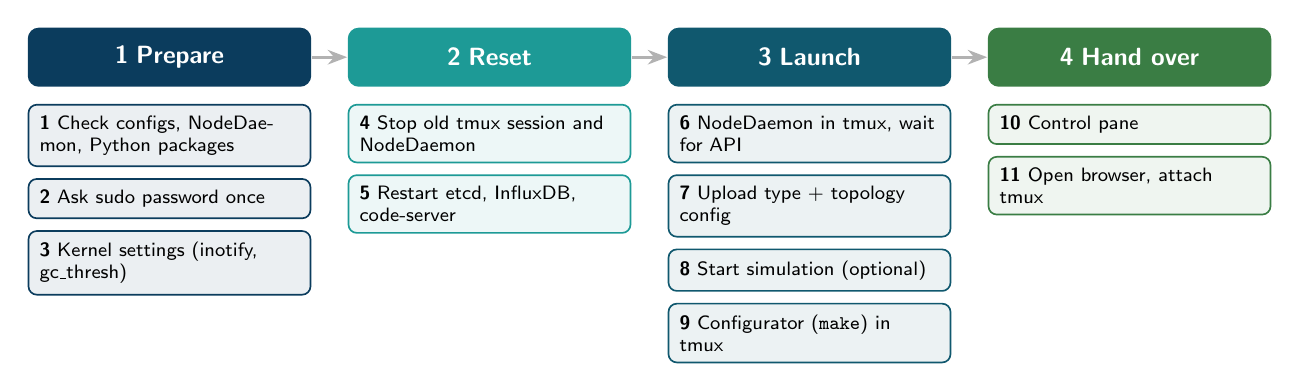
\begin{tikzpicture}[
  phase/.style={rectangle, rounded corners=4pt, fill=#1, text=white,
                font=\sffamily\bfseries\small, minimum width=3.6cm, minimum height=0.75cm},
  step/.style={rectangle, rounded corners=3pt, draw=#1, fill=#1!8, line width=0.6pt,
               font=\sffamily\scriptsize, text width=3.3cm, align=left, inner sep=4pt},
  arr/.style={-{Stealth[length=7pt]}, line width=1.2pt, color=gray!60},
  node distance=4pt]
  % Phase headers
  \node[phase=primary] (p1) {1\;Prepare};
  \node[phase=accent, right=0.45cm of p1] (p2) {2\;Reset};
  \node[phase=primary!70!accent, right=0.45cm of p2] (p3) {3\;Launch};
  \node[phase=tipc, right=0.45cm of p3] (p4) {4\;Hand over};
  \draw[arr] (p1) -- (p2); \draw[arr] (p2) -- (p3); \draw[arr] (p3) -- (p4);
  % Steps
  \node[step=primary, below=6pt of p1] (a1) {\textbf{1} Check configs, NodeDaemon, Python packages};
  \node[step=primary, below=of a1] (a2) {\textbf{2} Ask sudo password once};
  \node[step=primary, below=of a2] (a3) {\textbf{3} Kernel settings (inotify, gc\_thresh)};
  \node[step=accent, below=6pt of p2] (b1) {\textbf{4} Stop old tmux session and NodeDaemon};
  \node[step=accent, below=of b1] (b2) {\textbf{5} Restart etcd, InfluxDB, code-server};
  \node[step=primary!70!accent, below=6pt of p3] (c1) {\textbf{6} NodeDaemon in tmux, wait for API};
  \node[step=primary!70!accent, below=of c1] (c2) {\textbf{7} Upload type + topology config};
  \node[step=primary!70!accent, below=of c2] (c3) {\textbf{8} Start simulation (optional)};
  \node[step=primary!70!accent, below=of c3] (c4) {\textbf{9} Configurator (\texttt{make}) in tmux};
  \node[step=tipc, below=6pt of p4] (d1) {\textbf{10} Control pane};
  \node[step=tipc, below=of d1] (d2) {\textbf{11} Open browser, attach tmux};
\end{tikzpicture}
\end{center}

\begin{enumerate}
  \item \textbf{Checks first.} Confirms that both config files exist and are
    valid JSON, that \cmd{NodeDaemon} is present, and that the configurator's
    Python has its packages (Section~\ref{sec:python}). Nothing is changed
    until these pass.
  \item \textbf{sudo password.} Asks for it once and checks it.
  \item \textbf{Kernel settings,} set again on every run:
\begin{terminal}{kernel settings}
echo 4096  | sudo tee /proc/sys/fs/inotify/max_user_instances
echo 8192  | sudo tee /proc/sys/net/ipv4/neigh/default/gc_thresh1
echo 16384 | sudo tee /proc/sys/net/ipv4/neigh/default/gc_thresh2
echo 32768 | sudo tee /proc/sys/net/ipv4/neigh/default/gc_thresh3
\end{terminal}
  \item \textbf{Stops the previous run.} Closes any old \cmd{opensn} tmux
    session and stops any old \cmd{NodeDaemon} (SIGINT, then SIGKILL after
    15\,s if it's still running).
  \item \textbf{Dependency services.} Runs
    \cmd{scripts/start_depend_service.sh} from \cmd{daemon/opensn-daemon}, the
    folder its \cmd{../TopoConfigurators} path expects. This restarts the etcd,
    InfluxDB and code-server containers.
  \item \textbf{NodeDaemon.} Creates the tmux session and starts
    \cmd{sudo ./NodeDaemon} in pane 0 (\cmd{daemon}), then waits up to 60\,s
    for the API on port 8080 to respond.
  \item \textbf{Uploads the configs.} Sends the same API calls the web UI
    buttons make, and stops with an error if either upload is rejected:
\begin{terminal}{equivalent API calls}
curl -X POST -H 'Content-Type: application/json' \
     --data-binary @node_config.json  http://127.0.0.1:8080/api/emulation/update
curl -X POST -H 'Content-Type: application/json' \
     --data-binary @topology_config_today.json http://127.0.0.1:8080/api/emulation/topology
\end{terminal}
  \item \textbf{Starts the simulation (optional).} Calls
    \cmd{POST /api/emulation/start} only when \cmd{AUTO_START_EMULATION="yes"}.
  \item \textbf{Configurator.} Runs \cmd{make} (which runs
    \cmd{python3 main.py} with \cmd{ADDR=127.0.0.1 PORT=8080}) in pane 1
    (\cmd{configurator}), in the chosen Python environment.
  \item \textbf{Control pane.} Opens pane 2 (\cmd{control}) with the
    command to remove the dependency containers already typed in.
  \item \textbf{Browser and tmux.} Opens \url{http://127.0.0.1:8080} if a
    desktop session is available, prints a summary, and attaches to tmux.
\end{enumerate}

\begin{note}
The password reaches the NodeDaemon pane through a tmux buffer, so it is
never written to a file or shown on a command line.
\end{note}

%--------------------------------------------------------------------
\section{tmux session, logs and stopping}

Everything that keeps running is in the tmux session \cmd{opensn}, so you can
stop it from there. By default (\cmd{TMUX_LAYOUT="panes"}) all three open
together in one window, stacked as panes 0, 1 and 2; each pane's number and
name are shown in its top border.

\begin{center}
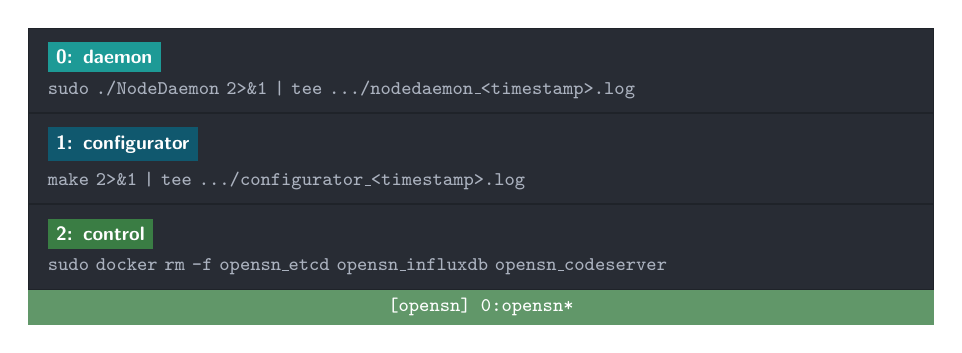
\begin{tikzpicture}[
  pane/.style={draw=termbar, fill=termbg, text=termfg, minimum width=11.5cm,
               minimum height=0.95cm, font=\ttfamily\scriptsize, align=left,
               text width=11cm, inner sep=5pt},
  bord/.style={fill=#1, text=white, font=\sffamily\scriptsize\bfseries,
               inner sep=2pt, anchor=north west}]
  \newcommand{\panelabel}[2]{\colorbox{#1}{\textcolor{white}{\sffamily\scriptsize\bfseries #2}}}
  \node[pane] (a) {\panelabel{accent}{0: daemon}\\[3pt] sudo ./NodeDaemon 2>\&1 | tee .../nodedaemon\_<timestamp>.log};
  \node[pane, below=0pt of a] (b) {\panelabel{primary!70!accent}{1: configurator}\\[3pt] make 2>\&1 | tee .../configurator\_<timestamp>.log};
  \node[pane, below=0pt of b] (c) {\panelabel{tipc}{2: control}\\[3pt] sudo docker rm -f opensn\_etcd opensn\_influxdb opensn\_codeserver};
  \node[fill=tipc!80, text=white, font=\ttfamily\scriptsize, anchor=north west,
        minimum width=11.5cm, inner sep=3pt] at (c.south west) {[opensn] 0:opensn*};
\end{tikzpicture}
\end{center}

\begin{nicetable}{@{}P{2.7cm}L P{4.5cm} P{2.7cm}@{}}
\headrow \thead{Pane} & \thead{Runs} & \thead{Log file} & \thead{To stop} \\
\cmd{daemon} (0)       & \cmd{sudo ./NodeDaemon} & \cmd{~/opensn/OpenSN-LeoSatellite/logs/} \cmd{nodedaemon_<timestamp>.log} & \kbd{Ctrl}+\kbd{C} \\
\cmd{configurator} (1) & \cmd{make}, which runs \cmd{python3 main.py} & \cmd{~/opensn/OpenSN-LeoSatellite/logs/} \cmd{configurator_<timestamp>.log} & \kbd{Ctrl}+\kbd{C} \\
\cmd{control} (2)      & A shell with the container-removal command already typed in & none & \kbd{Enter} \\
\end{nicetable}

With \cmd{TMUX_LAYOUT="windows"} the same three run as separate tmux windows
0, 1 and 2 instead.

The command waiting in the \cmd{control} pane:
\begin{terminal}{tmux: opensn:control}
sudo docker rm -f opensn_etcd opensn_influxdb opensn_codeserver
\end{terminal}

All logs go to \cmd{LOG_DIR} (Section~3). Output from \cmd{start_depend_service.sh} goes to
\cmd{~/opensn/OpenSN-LeoSatellite/logs/depend_<timestamp>.log}. Each run's logs share its timestamp,
so earlier runs aren't overwritten.

\subsection*{Useful tmux keys}
\begin{nicetable}{@{}P{5cm}L@{}}
\headrow \thead{Action} & \thead{Keys / command} \\
Reattach to the session      & \cmd{tmux attach -t opensn} \\
Go to pane 0, 1 or 2         & \kbd{Ctrl}+\kbd{b}\; then \kbd{q}, then \kbd{0} / \kbd{1} / \kbd{2} while the numbers show \\
Move to the pane above / below & \kbd{Ctrl}+\kbd{b}\; then \kbd{$\uparrow$} / \kbd{$\downarrow$} \\
Make a pane full screen (toggle) & \kbd{Ctrl}+\kbd{b}\; then \kbd{z} \\
Cycle pane arrangements      & \kbd{Ctrl}+\kbd{b}\; then \kbd{Space} \\
Scroll back through output   & \kbd{Ctrl}+\kbd{b}\; then \kbd{[}, arrows / \kbd{PgUp}, \kbd{q} to leave \\
Detach, leave everything running & \kbd{Ctrl}+\kbd{b}\; then \kbd{d} \\
\end{nicetable}

\begin{note}
\kbd{Ctrl}+\kbd{b} then \kbd{0}/\kbd{1}/\kbd{2} selects \emph{windows} in
plain tmux. The \cmd{~/.tmux.conf} on this host rebinds it to select
\emph{panes} 0/1/2 instead.
\end{note}

\begin{warning}
\kbd{Ctrl}+\kbd{C} goes to the selected pane (the one with the highlighted
border). Check which one is selected before pressing it.
\end{warning}

\begin{tip}
To stop everything: \kbd{Ctrl}+\kbd{C} in \cmd{configurator}, then
\kbd{Ctrl}+\kbd{C} in \cmd{daemon}, then \kbd{Enter} in \cmd{control}. You don't
have to stop anything before starting again: running the script again stops the
old session and \cmd{NodeDaemon} first.
\end{tip}

%--------------------------------------------------------------------
\section{Python environment}\label{sec:python}

The topology configurator needs \cmd{ephem}, \cmd{etcd3}, \cmd{loguru} and
\cmd{requests} (from \cmd{TopoConfigurators/Standard/requirements.txt}). On this
host only \cmd{~/python_venv} has them, so it is the default.

\begin{terminal}{opensn\_run.conf}
USE_VENV="yes"                  # "no" = use the system default python3
VENV_PATH="$HOME/python_venv"
\end{terminal}

\begin{nicetable}{@{}P{3.6cm}L@{}}
\headrow \thead{Setting} & \thead{What the configurator window runs} \\
\cmd{USE_VENV="yes"} & \cmd{source ~/python_venv/bin/activate} \mbox{\cmd{&& make}}, so \cmd{main.py} runs with the venv's \cmd{python3} \\
\cmd{USE_VENV="no"}  & \cmd{make} with the system \cmd{python3} \\
\end{nicetable}

\begin{warning}
The system Python doesn't have the packages yet. Before using
\cmd{USE_VENV="no"}, install them:
\begin{terminal}{ac@host: TopoConfigurators/Standard}
pip install -r requirements.txt
\end{terminal}
\end{warning}

Before asking for the password or restarting anything, the script checks that
the chosen Python can import all four packages. If \cmd{VENV_PATH} is wrong or
a package is missing, it stops with a message saying what to fix.

%--------------------------------------------------------------------
\section{Troubleshooting and notes}

\begin{nicetable}{@{}P{4.0cm}LL@{}}
\headrow \thead{Message or symptom} & \thead{Cause} & \thead{Fix} \\
\cmd{file not found} / \cmd{not valid JSON} & Wrong path, or a broken file, in \cmd{NODE_CONFIG} / \cmd{TOPO_CONFIG} & Correct the path in \cmd{opensn_run.conf}, or fix the file \\
\cmd{virtual env not found} & \cmd{VENV_PATH} doesn't point to a venv & Correct \cmd{VENV_PATH}, or set \cmd{USE_VENV="no"} \\
\cmd{configurator packages missing} & The chosen Python lacks the packages & \cmd{pip install -r requirements.txt} in that Python \\
\cmd{wrong sudo password} & Password mistyped & Run the script again \\
\cmd{Cannot create LOG_DIR} / \cmd{LOG_DIR is not writable} & No permission for the log folder & Set \cmd{LOG_DIR} in \cmd{opensn_run.conf} to a folder you can write to \\
\cmd{NodeDaemon API did not come up} & NodeDaemon failed or is still starting & \cmd{tmux attach -t opensn} and read the \cmd{daemon} window, or its log \\
\cmd{upload rejected} & NodeDaemon refused the config & The script prints the API response; check the file's contents \\
Browser doesn't open & No desktop session (for example, over SSH) & Open \url{http://127.0.0.1:8080} on the Linux host by hand \\
\end{nicetable}

\begin{note}
The launcher uses \cmd{~/opensn/OpenSN-LeoSatellite}. The separate
\cmd{~/opensn/OpenSN-Library} folder on the host isn't used. On this host,
\cmd{daemon/} and \cmd{TopoConfigurators/} are directly at the repo root, with
no \cmd{OpenSN-Library/} subfolder.
\end{note}

\begin{warning}
The script hasn't been run end to end yet. So far only its syntax and the
venv's packages have been checked.
\end{warning}

%--------------------------------------------------------------------
\clearpage
\appendix
\section{Configuration file: \texttt{opensn\_run.conf}}\label{app:conf}

\begin{codefile}{OpenSN-LeoSatellite/opensn\_run.conf}
# Settings for run_opensn.sh
# Relative paths are resolved against REPO.

# This file lives in the repo root next to run_opensn.sh, so REPO = that folder
REPO="$SCRIPT_DIR"

# Files uploaded the same way as the two web UI buttons
NODE_CONFIG="example/test_topologies/node_config.json"            # "Upload Type Configuration"
TOPO_CONFIG="example/test_topologies/topology_config_today.json"  # "Upload Topology Configuration"

# NodeDaemon API (same as the web UI)
API_URL="http://127.0.0.1:8080/api"
UI_URL="http://127.0.0.1:8080"

# Python for the TopoConfigurator (make -> python3 main.py)
# USE_VENV="yes" -> activate VENV_PATH before running make
# USE_VENV="no"  -> use the system default python3
USE_VENV="yes"
VENV_PATH="$HOME/python_venv"

TMUX_SESSION="opensn"
# TMUX_LAYOUT="panes"   -> all three in one window, split into panes (0 daemon, 1 configurator, 2 control)
# TMUX_LAYOUT="windows" -> one tmux window each
TMUX_LAYOUT="panes"
# Pane arrangement when TMUX_LAYOUT="panes": even-vertical (stacked), even-horizontal (side by side),
# main-horizontal (daemon large on top), main-vertical (daemon large on left), tiled (grid)
TMUX_PANE_LAYOUT="even-vertical"

# Where log files are written (created if missing).
# Absolute path, ~/..., or relative to REPO. Examples:
#   LOG_DIR="$REPO/logs"        (default: logs/ inside the repo)
#   LOG_DIR="$HOME/opensn_logs"
#   LOG_DIR="/data/opensn/logs"
# One-run override: LOG_DIR=/tmp/test_logs ./run_opensn.sh
LOG_DIR="$REPO/logs"

# yes = also press "Start Simulation" automatically after uploading
AUTO_START_EMULATION="yes"
# yes = open UI_URL in the browser (only if a desktop session is available)
OPEN_BROWSER="yes"
# yes = attach to the tmux session at the end
ATTACH="yes"
\end{codefile}

\section{Launcher script: \texttt{run\_opensn.sh}}\label{app:script}

\begin{codefile}{OpenSN-LeoSatellite/run\_opensn.sh}
#!/usr/bin/env bash
# One-shot launcher for OpenSN-LeoSatellite.
# Lives in the OpenSN-LeoSatellite repo root.
#   ./run_opensn.sh [config-file]           (default: opensn_run.conf next to this script)
#   NODE_CONFIG=... TOPO_CONFIG=... LOG_DIR=... ./run_opensn.sh    (env overrides the config file)
#
# tmux session (TMUX_LAYOUT=panes: one window, panes 0/1/2; =windows: one window each):
#   0 daemon        sudo ./NodeDaemon        (Ctrl-C stops it)
#   1 configurator  make (python main.py)    (Ctrl-C stops it)
#   2 control       shell with the "stop dependency containers" command pre-typed
set -euo pipefail

SCRIPT_DIR="$(cd "$(dirname "$0")" && pwd)"
CONF="${1:-$SCRIPT_DIR/opensn_run.conf}"

# Keep env overrides, then load config, then re-apply overrides
_env_node="${NODE_CONFIG:-}"; _env_topo="${TOPO_CONFIG:-}"; _env_log="${LOG_DIR:-}"
[[ -f "$CONF" ]] && source "$CONF" || { echo "Config not found: $CONF"; exit 1; }
[[ -n "$_env_node" ]] && NODE_CONFIG="$_env_node"
[[ -n "$_env_topo" ]] && TOPO_CONFIG="$_env_topo"
[[ -n "$_env_log"  ]] && LOG_DIR="$_env_log"

DAEMON_DIR="$REPO/daemon/opensn-daemon"
CONFIGURATOR_DIR="$REPO/TopoConfigurators/Standard"
S="$TMUX_SESSION"
TS="$(date +%Y%m%d_%H%M%S)"

# absolute as-is, ~/... -> $HOME/..., anything else relative to REPO
abspath() {
  case "$1" in
    /*)   echo "$1" ;;
    "~")  echo "$HOME" ;;
    "~/"*) echo "$HOME/${1#\~/}" ;;
    *)    echo "$REPO/$1" ;;
  esac
}
NODE_CONFIG="$(abspath "$NODE_CONFIG")"
TOPO_CONFIG="$(abspath "$TOPO_CONFIG")"
LOG_DIR="$(abspath "${LOG_DIR:-logs}")"
mkdir -p "$LOG_DIR" || { echo "Cannot create LOG_DIR: $LOG_DIR"; exit 1; }
[[ -w "$LOG_DIR" ]] || { echo "LOG_DIR is not writable: $LOG_DIR"; exit 1; }
LOG_DIR_Q="$(printf '%q' "$LOG_DIR")"   # shell-quoted, for commands typed into tmux

step() { echo -e "\n\033[1;36m==> $*\033[0m"; }
die()  { echo -e "\033[1;31mERROR: $*\033[0m" >&2; exit 1; }

for f in "$NODE_CONFIG" "$TOPO_CONFIG"; do
  [[ -f "$f" ]] || die "file not found: $f"
  jq empty "$f" 2>/dev/null || die "not valid JSON: $f"
done
[[ -x "$DAEMON_DIR/NodeDaemon" ]] || die "NodeDaemon not found in $DAEMON_DIR"

# ---- python environment for the configurator ----
if [[ "${USE_VENV:-no}" == "yes" ]]; then
  [[ -f "$VENV_PATH/bin/activate" ]] || die "virtual env not found: $VENV_PATH (set VENV_PATH or USE_VENV=\"no\" in $CONF)"
  PY="$VENV_PATH/bin/python3"
  PY_ACTIVATE="source '$VENV_PATH/bin/activate' && "
  echo "Configurator python: venv $VENV_PATH"
else
  PY="python3"
  PY_ACTIVATE=""
  echo "Configurator python: system $(command -v python3)"
fi
"$PY" -c 'import ephem, etcd3, loguru, requests' 2>/dev/null \
  || die "configurator packages missing in $PY (pip install -r $CONFIGURATOR_DIR/requirements.txt)"

# ---- sudo password (asked once; also fed to the NodeDaemon tmux pane) ----
step "sudo authentication"
read -rsp "[sudo] password for $USER: " SUDO_PW; echo
printf '%s\n' "$SUDO_PW" | sudo -S -p '' -v 2>/dev/null || die "wrong sudo password"

# ---- 1. kernel settings ----
step "Kernel settings"
echo 4096  | sudo tee /proc/sys/fs/inotify/max_user_instances
echo 8192  | sudo tee /proc/sys/net/ipv4/neigh/default/gc_thresh1
echo 16384 | sudo tee /proc/sys/net/ipv4/neigh/default/gc_thresh2
echo 32768 | sudo tee /proc/sys/net/ipv4/neigh/default/gc_thresh3

# ---- 2. stop previous run ----
step "Stopping previous run (tmux session '$S', NodeDaemon)"
tmux kill-session -t "$S" 2>/dev/null && echo "killed old tmux session" || true
if pgrep -x NodeDaemon >/dev/null; then
  sudo pkill -INT -x NodeDaemon || true
  for _ in $(seq 1 15); do pgrep -x NodeDaemon >/dev/null || break; sleep 1; done
  pgrep -x NodeDaemon >/dev/null && { echo "force killing NodeDaemon"; sudo pkill -KILL -x NodeDaemon || true; sleep 1; }
  echo "old NodeDaemon stopped"
else
  echo "no NodeDaemon running"
fi

# ---- 3. dependency services ----
step "Starting dependency services (log: $LOG_DIR/depend_$TS.log)"
( cd "$DAEMON_DIR" && ./scripts/start_depend_service.sh ) 2>&1 | tee "$LOG_DIR/depend_$TS.log"

# ---- 4. NodeDaemon in tmux ----
# TMUX_LAYOUT=panes   -> one window "opensn", panes 0 daemon / 1 configurator / 2 control
# TMUX_LAYOUT=windows -> separate windows daemon / configurator / control
LAYOUT="${TMUX_LAYOUT:-panes}"
[[ "$LAYOUT" == "panes" || "$LAYOUT" == "windows" ]] || die "TMUX_LAYOUT must be \"panes\" or \"windows\" (got \"$LAYOUT\")"

# new_pane <name> <dir> <pane to split after>  -> prints the new pane id
new_pane() {
  local id
  if [[ "$LAYOUT" == "panes" ]]; then
    id="$(tmux split-window -d -v -t "$3" -c "$2" -P -F '#{pane_id}')"
    tmux select-layout -t "$3" "${TMUX_PANE_LAYOUT:-even-vertical}"
  else
    id="$(tmux new-window -d -t "$S" -n "$1" -c "$2" -P -F '#{pane_id}')"
  fi
  tmux select-pane -t "$id" -T "$1"
  echo "$id"
}

step "Starting NodeDaemon in tmux ($LAYOUT, log: $LOG_DIR/nodedaemon_$TS.log)"
[[ "$LAYOUT" == "panes" ]] && WIN_NAME="opensn" || WIN_NAME="daemon"
P_DAEMON="$(tmux new-session -d -s "$S" -n "$WIN_NAME" -c "$DAEMON_DIR" -x 200 -y 60 -P -F '#{pane_id}')"
tmux select-pane -t "$P_DAEMON" -T daemon
# Pane names in the borders; keep programs from renaming them
tmux set -w -t "$P_DAEMON" pane-border-status top
tmux set -w -t "$P_DAEMON" pane-border-format " #{pane_index}: #{pane_title} "
tmux set -w -t "$P_DAEMON" allow-set-title off 2>/dev/null || true
tmux send-keys -t "$P_DAEMON" "sudo ./NodeDaemon 2>&1 | tee $LOG_DIR_Q/nodedaemon_$TS.log" Enter
# Answer the sudo prompt in the pane via a tmux buffer (password never appears on a command line)
for _ in $(seq 1 10); do
  sleep 0.5
  if tmux capture-pane -p -t "$P_DAEMON" | grep -qi 'password for'; then
    printf '%s' "$SUDO_PW" | tmux load-buffer -b pw -
    tmux paste-buffer -d -b pw -t "$P_DAEMON"
    tmux send-keys -t "$P_DAEMON" Enter
    break
  fi
done
unset SUDO_PW

echo -n "waiting for API $API_URL "
for i in $(seq 1 60); do
  curl -fs "$API_URL/emulation/" >/dev/null 2>&1 && { echo " up"; break; }
  echo -n "."; sleep 1
  [[ $i == 60 ]] && die "NodeDaemon API did not come up. Check: tmux attach -t $S"
done

# ---- 5. upload configs (same calls as the web UI buttons) ----
upload() { # $1 = endpoint, $2 = file, $3 = label
  local resp
  resp="$(curl -fsS -X POST -H 'Content-Type: application/json' --data-binary @"$2" "$API_URL/emulation/$1")" \
    || die "$3 upload failed (HTTP error)"
  [[ "$(jq -r '.code' <<<"$resp" 2>/dev/null)" == "0" ]] || die "$3 upload rejected: $resp"
  echo "$3 uploaded: $(basename "$2")"
}
step "Uploading configuration files"
upload update   "$NODE_CONFIG" "Type configuration"
upload topology "$TOPO_CONFIG" "Topology configuration"

if [[ "$AUTO_START_EMULATION" == "yes" ]]; then
  step "Starting emulation"
  curl -fsS -X POST "$API_URL/emulation/start"; echo
fi

# ---- 6. configurator in tmux ----
step "Starting configurator in tmux (log: $LOG_DIR/configurator_$TS.log)"
P_CONF="$(new_pane configurator "$CONFIGURATOR_DIR" "$P_DAEMON")"
tmux send-keys -t "$P_CONF" "${PY_ACTIVATE}make 2>&1 | tee $LOG_DIR_Q/configurator_$TS.log" Enter

# ---- 7. control pane/window ----
P_CTRL="$(new_pane control "$DAEMON_DIR" "$P_CONF")"
tmux send-keys -t "$P_CTRL" "# Stop: Ctrl-C in 'daemon' and 'configurator'; press Enter here to remove dependency containers" Enter
tmux send-keys -t "$P_CTRL" "sudo docker rm -f opensn_etcd opensn_influxdb opensn_codeserver"
tmux select-window -t "$P_DAEMON"
tmux select-pane -t "$P_DAEMON"

# ---- 8. browser ----
if [[ "$OPEN_BROWSER" == "yes" && -n "${DISPLAY:-}${WAYLAND_DISPLAY:-}" ]] && command -v xdg-open >/dev/null; then
  xdg-open "$UI_URL" >/dev/null 2>&1 &
fi

step "Done"
echo "Simulator UI : $UI_URL"
if [[ "$LAYOUT" == "panes" ]]; then
  echo "tmux session : tmux attach -t $S   (panes 0 daemon / 1 configurator / 2 control; Ctrl-b q then number, Ctrl-b z zoom, Ctrl-b d detach)"
else
  echo "tmux session : tmux attach -t $S   (windows: Ctrl-b n next / Ctrl-b w list, Ctrl-b d detach)"
fi
echo "Logs         : $LOG_DIR/*_$TS.log"

if [[ "$ATTACH" == "yes" && -t 1 ]]; then
  if [[ -n "${TMUX:-}" ]]; then
    tmux switch-client -t "$S"      # already inside tmux
  else
    tmux attach -t "$S"
  fi
fi
\end{codefile}

\end{document}
